%% https://github.com/tbielawa/PAD-XMPP/blob/master/Graph/ConnectionStates.png
\documentclass{article}
%\usepackage{fullpage}
\usepackage{booktabs}
\usepackage{amsmath}
\usepackage{amssymb}
\usepackage[noend]{algorithmic}
\usepackage[nothing]{algorithm}
\usepackage{tikz}
\usepackage{latexsym}
\usepackage{float}
\usepackage{hyperref}
\usetikzlibrary{arrows,automata}
\providecommand{\e}[1]{\ensuremath{\times 10^{#1}}}
\renewcommand{\thealgorithm}{}
\renewcommand*{\thefootnote}{[\arabic{footnote}]}
\title{CS 544: Computer Networks \\ Multicast Multi-User Chat Protocol}
\author{Brian Balderston, Dustin Ingram, Clint Kirberger, Ben Schilke}
\begin{document}
\maketitle
\begin{abstract}
Multicast Multi-User Chat is a distributed, non-reliable application-layer
protocol that uses UDP at the transport layer and provides multi-user chat room
creation, discovery, and the exchange of user presence information and messaging
without a central server. 
\end{abstract}
\section{Introduction}
Multicast Multi-User Chat is a distributed, non-reliable application-layer
protocol that uses UDP at the transport layer and provides multi-user chat room
creation, discovery, and the exchange of user presence information and messaging
without a central server. 

A client can join a chat room by name, which is hashed to a specific multicast
channel within a given range of channels, excluding those already in use. The
client then sends messages intended for that multi-user chat on the channel
produced by the hashing algorithm.

The protocol is distributed and decentralized by using a classical flooding
algorithm to forward non-duplicate messages.

\subsection{Terminology}
\begin{itemize}
\item \textbf{Control Channel}: a fixed port for the sending of messages, such
as room creation and detection, that must reach all clients on the network
\item \textbf{MUC Channel}: a dynamic port that is actively being used for chat
by one or more clients, and which all clients are aware they must forward
traffic for
\item \textbf{MUC}: a Multi-User Chat, a shared ``chat room'' between multiple
clients.
\item \textbf{MUC Message}: a message from one client to all clients in the MUC
\item \textbf{Direct Message}: a message from one client that is forwarded to
all clients in the MUC but that is directed to one client in particular - MUC
software implementations may choose to not display messages not directed at the
active user
\end{itemize}
\section{Message Types}

Protocol messages are JSON (JavaScript Object Notation) collections of
name/value pairs. JSON was chosen because it is easy for both machines and
humans to read and parse. 

The primitive data types used in the protocol are $\langle\text{integer}\rangle$, a 32-bit signed
two's complement integer, $\langle\text{long-integer}\rangle$, a 64-bit signed two's complement
integer, and $\langle\text{string}\rangle$, a sequence of characters in the UTF-16 format.

The following compound types are also provided:
\begin{align*}
\langle integer\text{-}list\rangle &\rightarrow \langle integer \rangle |
\langle integer \rangle , \langle integer\text{-}list \rangle \\
\langle certificate\rangle  &\rightarrow \{ \text{`certificate'} : \langle
string\rangle
, \text{`format'} : \langle string\rangle \} \\
\langle certificate\text{-}list\rangle &\rightarrow \langle certificate
\rangle | \langle certificate \rangle, \langle
certificate\text{-}list\rangle
\end{align*}
All messages are of the format 
\begin{align*}
\{\text{`uid'} : \langle uid\rangle, \text{`action'} : \langle action\rangle \}
\end{align*}
where an action may be:
\begin{align*}
\langle action \rangle\rightarrow&\langle list\text{-}rooms\rangle|\langle
use\text{-}rooms \rangle|\langle message\rangle| \\
&\langle presence\rangle|\langle timeout \rangle|\langle preserve\rangle 
\end{align*}
and `uid' is an unique identifier for each message sent by a client and 
\begin{align*}
\langle uid\rangle\rightarrow\langle long\text{-}integer\rangle
\end{align*}
`certificate' is a public key certificate, and `format' specifies the
certificate format, such as PGP or X.509. This allows the clients to use both
self-signed and certificate-authority (CA) issued certificates.
\subsection{Unique IDs (UIDs)}
For the multicast flooding algorithm, each node must have a way of tracking of
each message it has forwarded, to avoid forwarding them again. Simply requiring
the clients to keep the last n messages is insufficient, as there is no method
to distinguish between duplicates and messages that are new but the same as old
messages (such as when a room gets re-created or a message with the same
body/from fields). Thus the protocol will require unique message ID numbers;
each client can generate a unique ID for each message it creates, and every
other client can use this ID to determine if the message is a duplicate or not.
This must be an attribute of every message and each client would have a history
of message IDs seen. Clients must also store an MD5 hash of the message with the
ID, so that IDs may eventually be reused. So the client receives
\begin{align*}
\{\text{`uid'}:\text{`}X\text{'},\langle Y\rangle\}
\end{align*}
where $\langle Y\rangle$  is a collection of key/value pairs, and only forwards
it once, but would forward 
\begin{align*}
\{\text{`uid'}:\text{'}X\text{'},\langle Z\rangle\}
\end{align*}
if $Y$ has a different hash than $Z$, and so on.

From a security perspective, one can't rely on any particular behavior (globally
unique ids) from a client. For a sequence of packets sent by a given client, the
UIDs need to be unpredictable, or a malicious client can stop another client's
packets from being forwarded. We have to assume the only uniqueness comes from
the client's ability to generate a random sequence of numbers. We do not specify
the ID generation algorithm for clients.
\subsection{Control Messages}

The $list\text{-}rooms$ action is used by clients to update channel use information. If
the optional collection of rooms is not included, this signals that the client
wants to know about all channels in use. If a collection of rooms is provided,
the client wishes to know the status of just those channels. list-rooms takes
the form:
\begin{align*}
\langle list\text{-}rooms\rangle  \rightarrow \text{`list-rooms'} , [ \text{`rooms'} :
[\langle integer\text{-}list\rangle ] ]
\end{align*}

The $use\text{-}rooms$ action is used to reply to a $list\text{-}rooms$ action. Clients will
either reply with a collection of all channels they know are in use or the
subset of channels in use that were asked about in the original
$list\text{-}rooms$
action. In addition, $use\text{-}rooms$ is also used to create a new room. The
syntax of $use\text{-}rooms$ is:
\begin{align*}
\langle use\text{-}rooms\rangle \rightarrow \text{`use-rooms'}, \text{`rooms'} :
[\langle integer\text{-}list\rangle ]
\end{align*}

The timeout action is used by clients to find channels clients are no longer
actively using to chat, and thus whose allocated resources can be freed. The
timeout is used to ask the other clients which of the provided rooms they are
using: 
\begin{align*}
\langle timeout\rangle  \rightarrow \text{`timeout'}, \text{`rooms'} : [\langle
integer\text{-}list\rangle ]
\end{align*}
The preserve action is used to reply to a timeout action, indicating that
clients should continue to forward traffic for the included rooms:
\begin{align*}
\langle preserve\rangle  \rightarrow \text{`preserve'}, \text{`rooms'} :
[\langle integer\text{-}list\rangle ]
\end{align*}
\subsection{Presence Messages}

\begin{align*}
\langle poll\text{-}presence\rangle  \rightarrow& \text{`poll-presence'} \\
\langle presence\rangle  \rightarrow& \text{`presence'} , \text{`from'} :
\langle string\rangle, \text{`status'} : \langle status\rangle \\
& [ , \text{`keys'} : [\langle certificate\text{-}list\rangle ] ] \\
\langle status\rangle  \rightarrow& \text{`online'} | \text{`offline'}
\end{align*}
\subsection{Chat Messages}

A chat room message action must carry a `from' field, which is a nickname that
identifies the sender, and a `body' field that carries the user's input.
Messages can also optionally contain a `to' value, for which clients can choose
to hide from the user messages not meant for them. Messages can also be
optionally encrypted with the public key certificate specified by `key'. Using
`to' and `key' together allows clients to avoid checking the `key' against their
own keystore, as they will know the messages was not directed at them. The
formal specification for message is:
\begin{align*}
\langle message\rangle  \rightarrow& \text{`message'} , \text{`from'} : \langle
string\rangle  , \text{`body'} : \langle string\rangle \\
&[ , \text{`to'} :
\langle string\rangle  ] [ , \text{`key'}: \langle certificate\rangle  ]
\end{align*}
\section{States of a Node}
See included diagrams for full-size DFAs of a control channel and a MUC channel.
\begin{center}
\scalebox{.38}{
    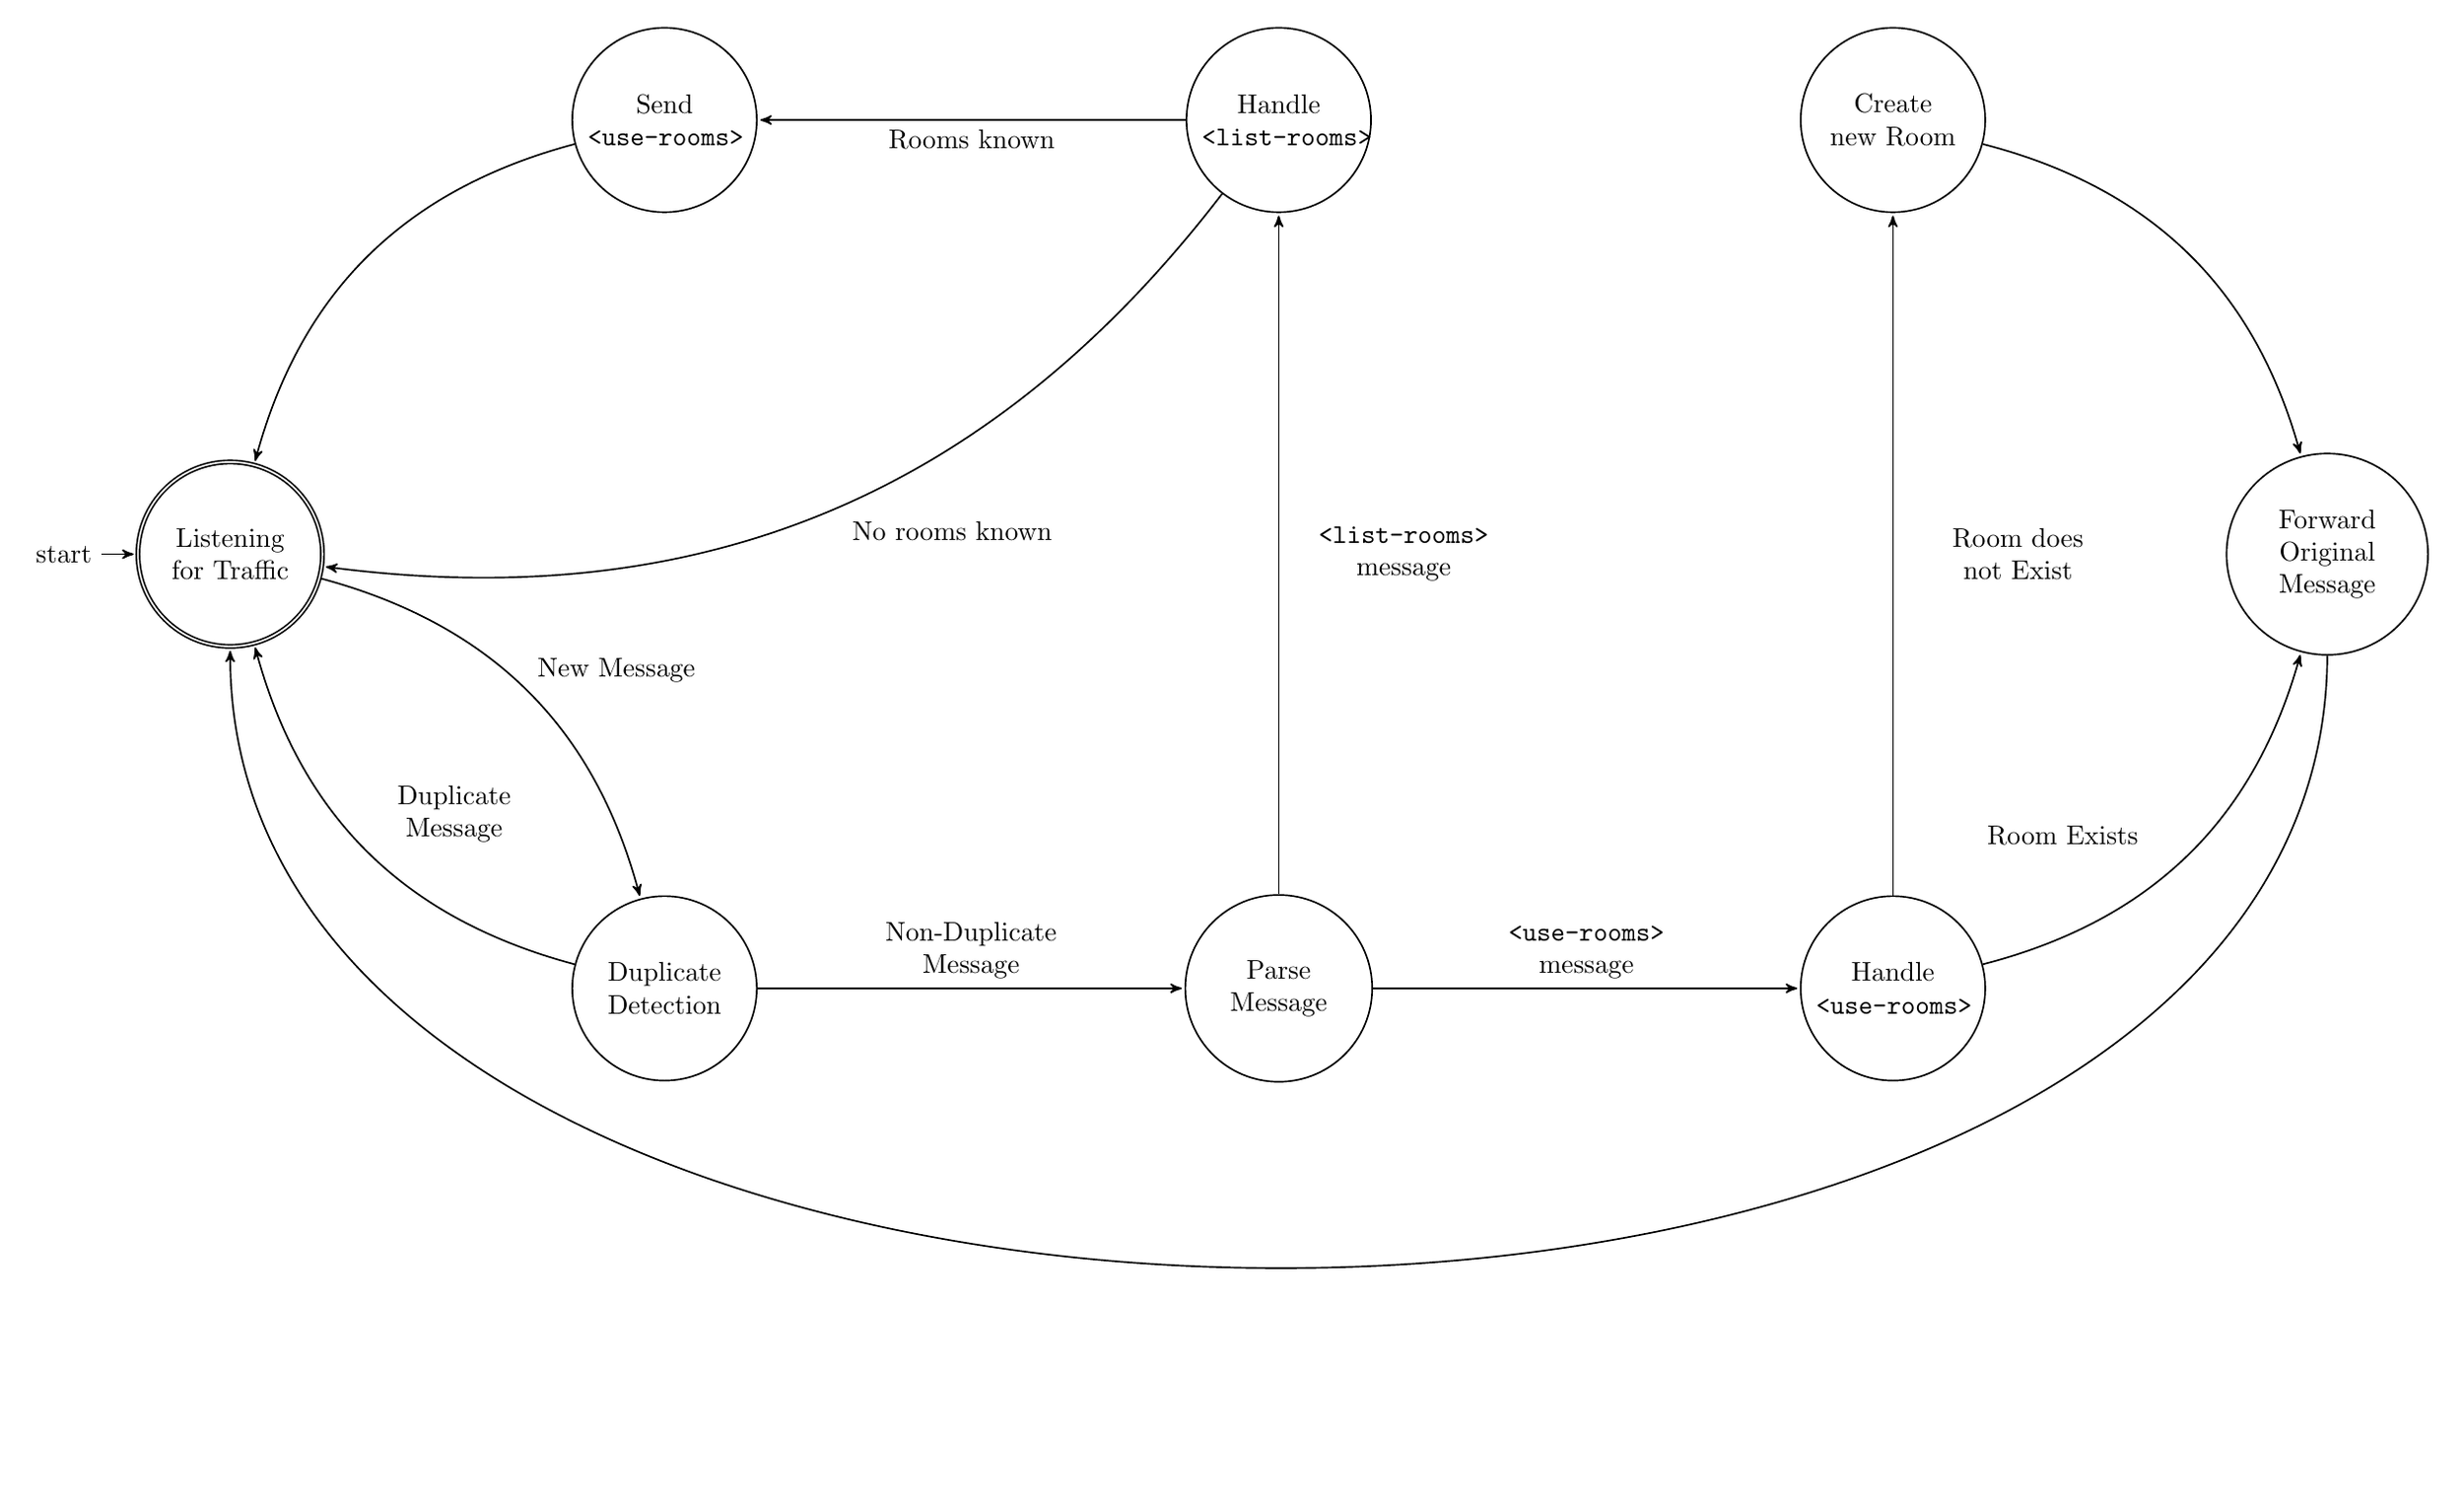
\begin{tikzpicture}[->,>=stealth',shorten >=1pt,auto,semithick, node
    distance=8cm]
      \node[state, initial, text width=2cm, align=center, accepting] (q1) at (0,0)
        {Listening for Traffic};
      \node[state, text width=2cm, align=center, below right of=q1] (q2)
        {Duplicate Detection};
      \node[state, text width=2cm, align=center, right of=q2] (q8)
        {Parse Message};
      \node[state, text width=2cm, align=center, above right of=q1] (q14)
        {Send \texttt{<use-rooms>}};
      \node[state, text width=2cm, align=center, right of=q14] (q4)
        {Handle \texttt{<list-rooms>}};
      \node[state, text width=2cm, align=center, right of=q8] (q6)
        {Handle \texttt{<use-rooms>}};
      \node[state, text width=2cm, align=center, right of=q4] (q7)
        {Create new Room};
      \node[state, text width=2cm, align=center, above right of=q6] (q10)
        {Forward Original Message};

      \path
            (q1) edge[bend left] node {New Message} (q2)
            (q2) edge[text width=2cm, align=center, bend left] node[above right] {Duplicate Message} (q1)
            (q2) edge[text width=3cm, align=center] node {Non-Duplicate Message} (q8)
            (q8) edge[text width=3cm, align=center] node[right] {\texttt{<list-rooms>} message} (q4)
            (q8) edge[text width=3cm, align=center] node {\texttt{<use-rooms>} message} (q6)
            (q6) edge[bend right, text width=3cm, align=center] node {Room Exists} (q10)
            (q6) edge[text width=3cm, align=center] node[right] {Room does not Exist} (q7)
            (q4) edge[text width=3cm, align=center, bend left] node {No rooms known} (q1)
            (q4) edge[text width=3cm, align=center] node {Rooms known} (q14)
            (q7) edge[bend left, text width=3cm, align=center] node {} (q10)
            (q14) edge[bend right, text width=3cm, align=center] node {} (q1)
            (q10) edge[text width=3cm, align=center, bend left, in=90, out=90] node {} (q1)
            ;
    \end{tikzpicture}

}
\end{center}

\begin{center}
\scalebox{.38}{
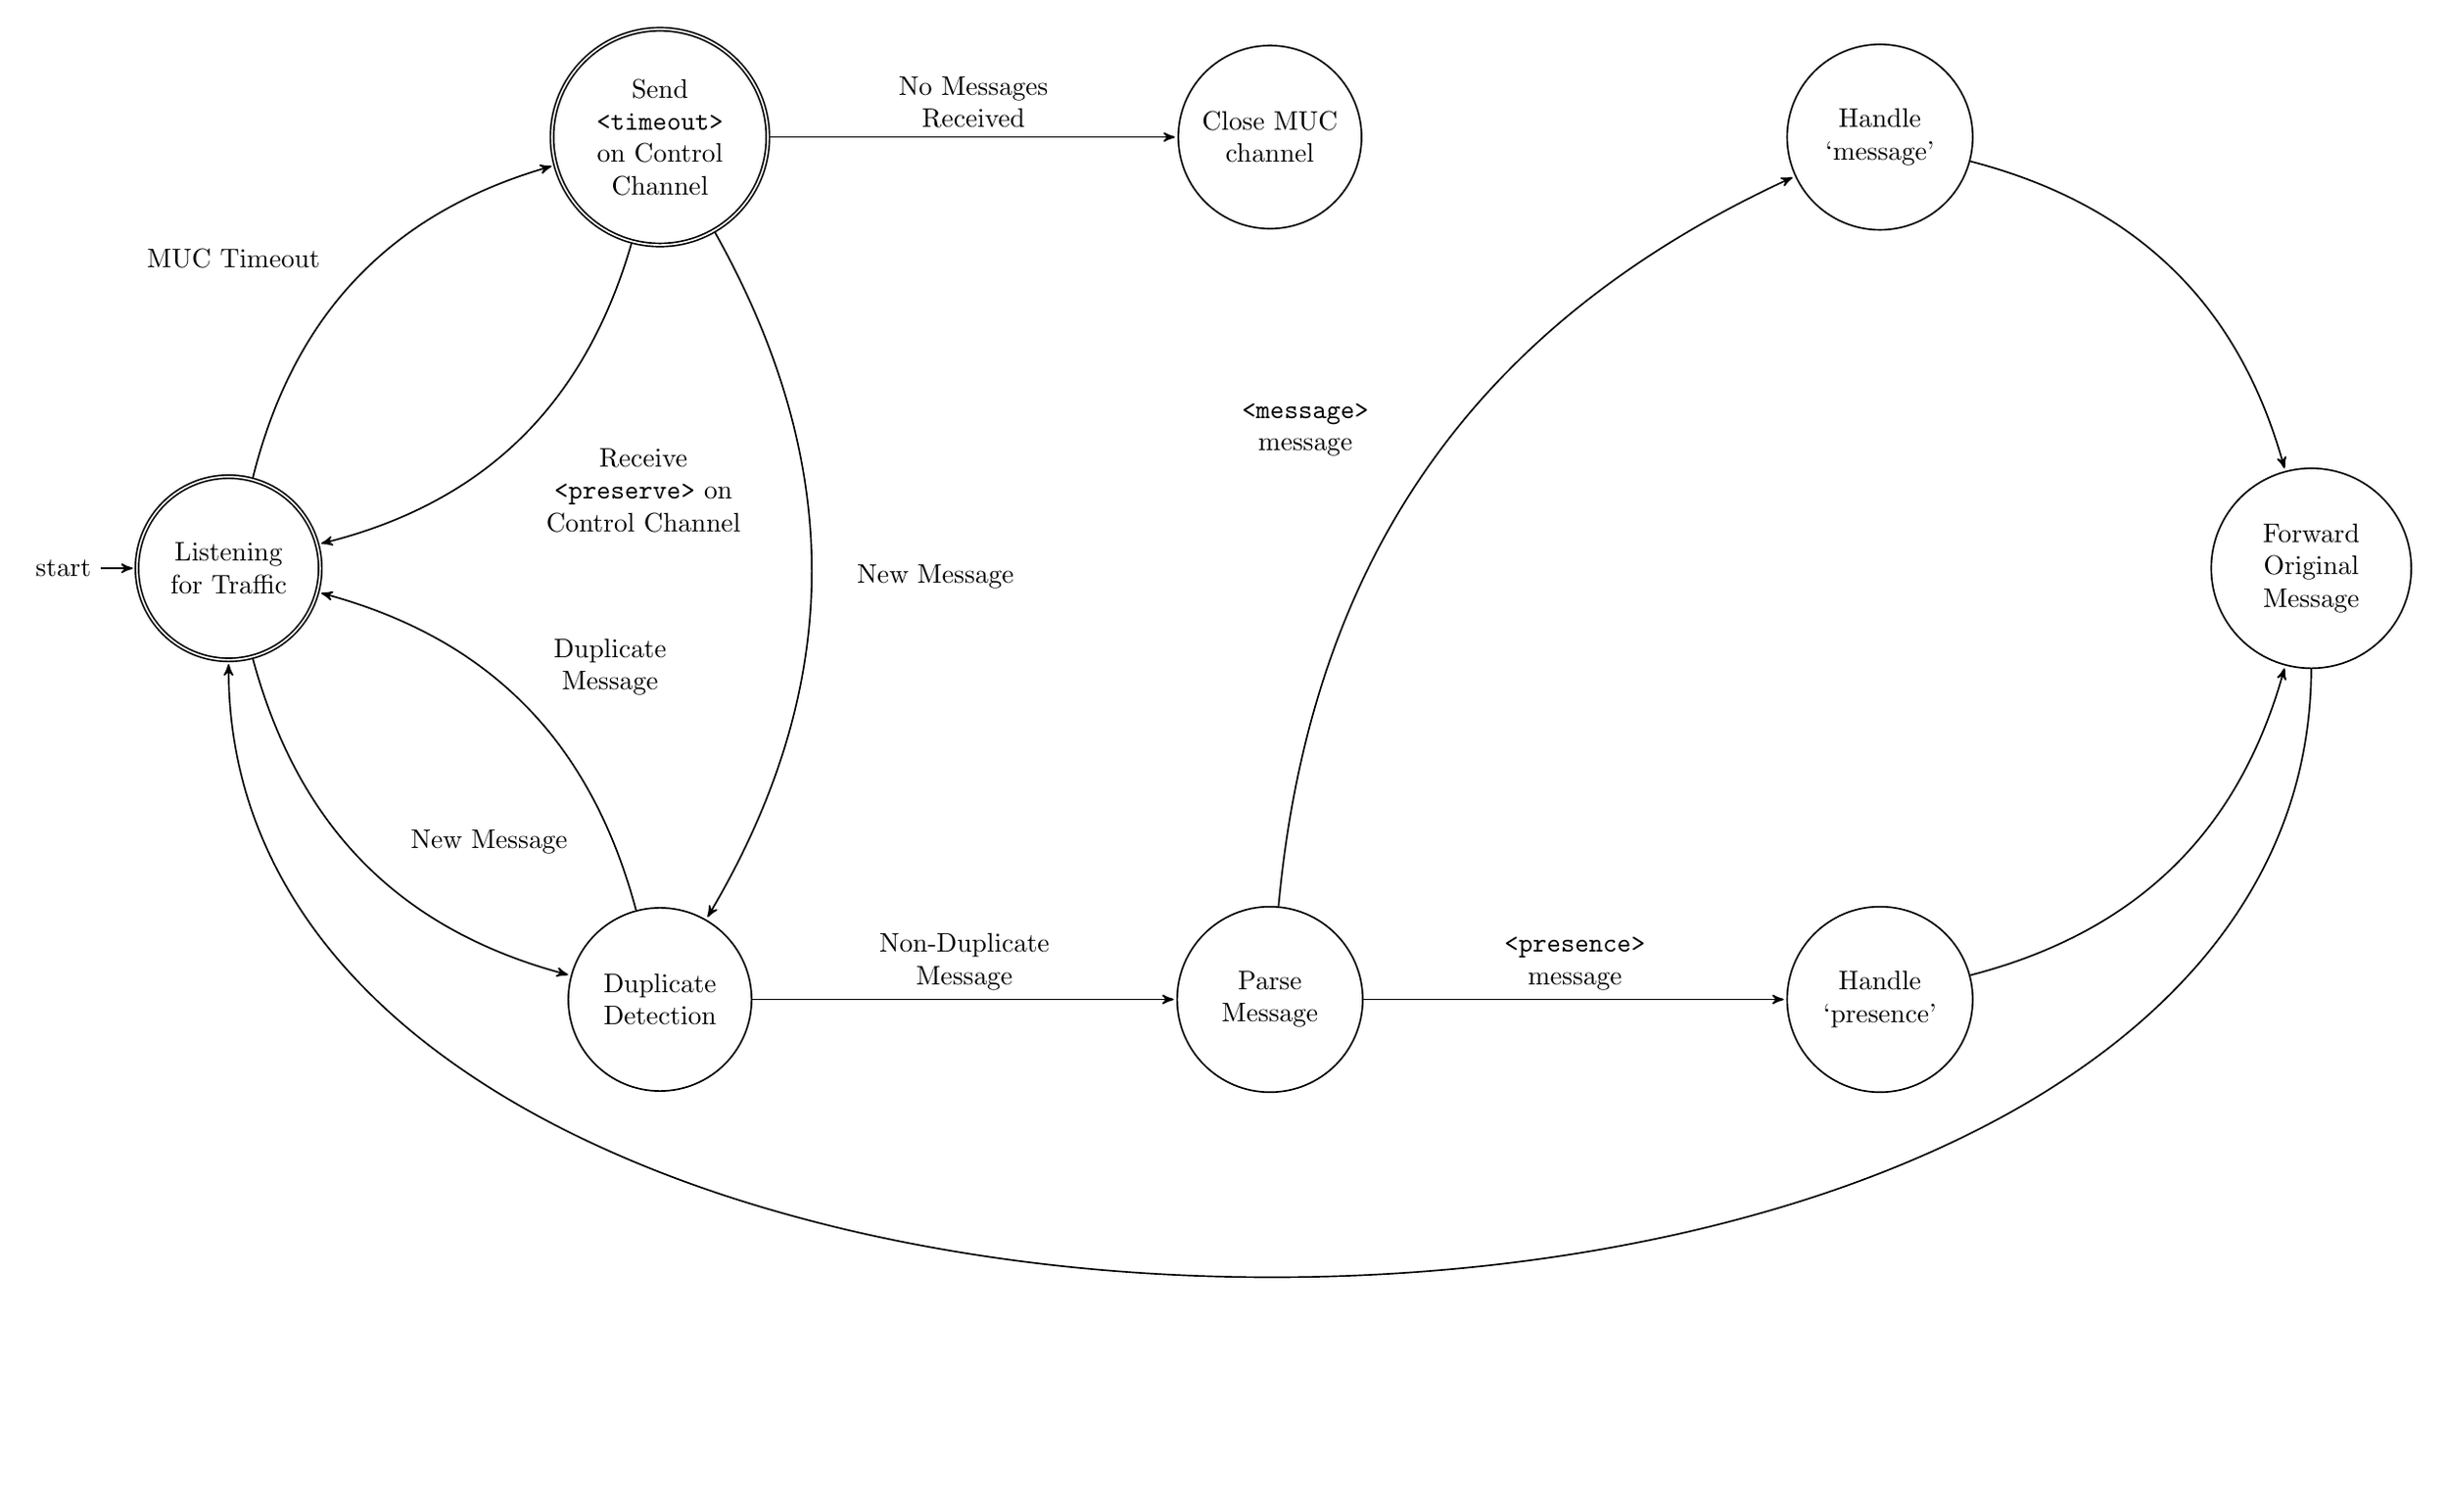
\begin{tikzpicture}[->,>=stealth',shorten >=1pt,auto,semithick, node
    distance=8cm]
      \node[state, initial, text width=2cm, align=center, accepting] (q1) at (0,0)
        {Listening for Traffic};
      \node[state, text width=2cm, align=center, above right of=q1, accepting] (q8)
        {Send \texttt{<timeout>} on Control Channel};
      \node[state, text width=2cm, align=center, right of=q8] (q9)
        {Close MUC channel};
      \node[state, text width=2cm, align=center, below right of=q1] (q2)
        {Duplicate Detection};
      \node[state, text width=2cm, align=center, right of=q2] (q3)
        {Parse Message};
      \node[state, text width=2cm, align=center, right of=q3] (q6)
        {Handle `presence'};
      \node[state, text width=2cm, align=center, right of=q9] (q5)
        {Handle `message'};
      \node[state, text width=2cm, align=center, below right of=q5] (q10)
        {Forward Original Message};

      \path
            (q1) edge[text width=3cm, bend right, align=center] node {New Message} (q2)
            (q2) edge[text width=2cm, bend right, align=center] node[above right] {Duplicate Message} (q1)
            (q2) edge[text width=3cm, align=center] node {Non-Duplicate Message} (q3)
            (q3) edge[text width=3cm, align=center, bend left] node {\texttt{<message>} message} (q5)
            (q3) edge[text width=3cm, align=center] node {\texttt{<presence>} message} (q6)
            (q6) edge[text width=3cm, align=center, bend right] node {} (q10)
            (q1) edge[text width=3cm, align=center, bend left] node {MUC Timeout} (q8)
            (q8) edge[text width=3cm, align=center] node {No Messages Received} (q9)
            (q8) edge[text width=3cm, align=center, bend left] node {Receive
            \texttt{<preserve>} on Control Channel} (q1)
            (q8) edge[text width=3cm, align=center, bend left] node {New Message} (q2)
            (q5) edge[text width=3cm, align=center, bend left] node {} (q10)
            (q10) edge[text width=3cm, align=center, bend left, in=90, out=90] node {} (q1)
            ;
    \end{tikzpicture}

}
\end{center}
\section{Joining a Network}

\subsection{Discovering Peers}

A control channel on a fixed port (31941) is used to announce the creation of
each new room, by specifying a new channel that clients should listen on and
forward traffic. When a new client connects to the network, they send a message
on the control channel announcing their existence, and its neighbors inform the
client of the channels they know about.
Version Negotiation

Due to the nature of Multicast IP, the protocol will indiscriminately send it's
multicast messages to all clients on a LAN. Since any version of the protocol
will use the same port for the control channel, and could feasibly use the same
ports as MUC channels, performing actual version negotiation would not reduce or
eliminate the possible receipt of messages using different versions. Therefore,
it shall be the responsibility of all implementations to ignore any message
which is not properly formatted or of a type described in the version it is
using. Similarly, it shall be the responsibility of all future versions to offer
full backwards compatibility, or fully ignore messages from incompatible
versions.

\section{Joining a MUC}

\subsection{Channel Hash Algorithm}

The protocol uses a double hashing algorithm: it uses one hash value as a
starting point and repeatedly steps forward an interval determined by second
hash function until an unused port is found. A good hash function will map
inputs evenly over the output range, as the computational cost of hashing
increases with the number of collisions. Double hashing minimizes collisions
more effectively than linear or quadratic probing strategies. The $i$-th position
of given value $x$, in a range of size n is then 
\begin{align*}
F(x,i) = G(x) + i * H(x)\mod{n}
\end{align*}
Here, $G$
and $H$ should each produce a 32-bit signed two's complement integer (twice the
range of dynamic ports) using the concatenated first four bytes of the MD5
cryptographic hash for $G$ and SHA-1 for $H$.

Limiting a channel to one chat room helps scale the protocol as high amount of
UDP traffic on a single port can quickly experience data loss and congestion. It
does limit the number of possible rooms, but each channel will have better
performance because there is less contention for bandwidth. We see this as a
minor drawback, as the number of dynamic ports is large on a modern OS (16,384
in the IANA range, used by Windows, and 28,233 on some Linux kernels).
Channel Announcement

To announce the creation of a new MUC room (and thus, a new MUC channel) to all
peer nodes, a client should send an announcement message on the control channel 
Sending a MUC Message

\subsection{Addressing}

Addressing in this protocol is not addressing in the typical sense. Because MUC
messages are delivered to all clients in the MUC, and MUC channels are
restricted to their individual ports, there is no need to specifically address a
message to a client or MUC. Instead, clients must specify a ``from'' attribute, to
add organization to chat messages and support for presence messages.

Alternatively, the protocol can support direct messaging by specifying a ``to''
attribute. However, there is no acknowledgement for any messages, including
direct messages, and mis-addressed messages will simply be ignored by all
clients.

\subsection{Address Collisions}
Address collisions are allowed by the protocol. Although this may present an
issue with presence information if two distinctly different clients attempt to
use the the same address
Message Text Encoding

All messages are encoded in UTF-16, a character encoding for Unicode that uses
one or two 16-bit codes per character.
Hard Message Size Limit

A UDP datagram has a 16-bit length field and a 8 byte header, which allows for a
theoretical data length of $65,535 - 8 = 65,527$ bytes. However, the practical
limit for the message length is imposed by the underlying IPv4 protocol, which
has a 20 byte header, and is thus $65,527 - 20 = 65,507$ bytes. $65,507$ bytes can
represent between $2,047$ to $4,095$ UTF-16 characters, which is considerably longer
than the typical messages expected to be sent in practice, and thus the
protocol will not perform fragmentation and reassembly.

\subsection{Peer-to-peer Message Delivery}

The flooding algorithm is simple, forwarding all non-duplicate messages to all
single-hop neighbors.

\subsection{MUC Maintenance}

\subsubsection{Timeout/Shutdown}

Each client sets random timer for between 5-10 minutes after receiving a message
on port $N$. When a client doesn't see any further traffic on port $N$ before the
timer expires, and it isn't in the room for Port $N$ itself, it sends out a
`timeout' action on the control channel. Any client that see the `timeout'
action stops its own timer. If any client responds to the `timeout' poll before
a timeout period of 60 seconds, all clients keep port $N$ open and reset their
timers. If no clients
respond, all clients shut down on port $N$.

\section{Reliability Considerations}

Since the protocol uses UDP, which makes no promise of reliability, the
reliability of the protocol is a function of the number of peers. Clients
forward messages even for rooms they're not in and thus adding or removing peers
from the network can alter the reliability of any given chat room.

\section{Security Considerations}

Messages sent over MUC will not be secure by default. This creates the risk that
a man-in-the-middle attack could read message intended for someone else.  We
will allow clients to send their certificate if they have one, allowing for
others to send messages encrypted with the public key they get from the
certificate. The certificates could be authorized by Certificate Authorities or
they could be issued by one of the web of trust organizations (e.g. PGP, GnuPG,
OpenPGP, etc.). Certificates can also be used to authenticate messages coming
from the owner of the public key are actually being sent by the owner of the
certificate, which could be useful in the context of MUC.  (We considered using
the symmetric key encryption and encrypting the entire channel, but this seems
to be too complicated to implement for this project.)

Another security vulnerability is the possibility that a client could try
opening a large number of rooms or sending a large number of messages, with the
aim of using up connected clients' resources, or the MUC network's bandwidth.
This could be prevented by limiting each client to creating no more than x
number of rooms in a 24-hour period, and preventing the client from sending out
y number of messages in a 60-second period.  This could add a lot of complexity
because it would require adding timers to the client for both actions (creating
rooms and sending messages) and it wouldn't prevent someone who had figured out
the MUC message protocol from sending their own messages without these
limitations.

\section{Detailed Examples}

Sample network configuration for these examples is as follows:

\begin{center}
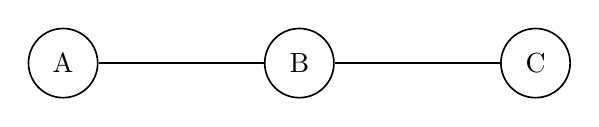
\begin{tikzpicture}[-,>=stealth',auto,semithick, node
distance=8cm]
    \node[state] (A) at (0,0) {A};
    \node[state] (B) at (3,0) {B};
    \node[state] (C) at (6,0) {C};

    \path
        (A) edge node {} (B)
        (B) edge node {} (C);
\end{tikzpicture}
\end{center}

\subsection{Control Messages}
\subsubsection{Room Discovery}

In this example, Client A knows about no rooms, and Client B responds with the
rooms it knows about:
\begin{align*}
\textbf{Client A}:& \text{\{ `action' : `list-rooms' \}} \\
\textbf{Client B}:& \text{\{ `action' : `use-rooms', `rooms' : [51200, 45235,
656] \}}
\intertext{or, in this example, Client A knows about two rooms. Client B is using these two
rooms, plus a third that Client A did not know about:}
\textbf{Client A}:& \text{\{ `uid' : `X', `action' : `list-rooms', `rooms' :
[51200, 45235] \}}\\
\textbf{Client B}:& \text{\{ `uid' : `Y', `action' : `use-rooms', `rooms' :
[51200, 45235, 60056] \}}
\end{align*}

\subsubsection{MUC Room Creation}

In this example, Client A creates a room. The `use-rooms' message then
propagates through the network as it is repeated by clients B and C:
\begin{align*}
\textbf{Client A}: \text{\{ `uid' : `X', `action' : `use-rooms', `rooms' :
[51200] \}}\\
\textbf{Client B}: \text{\{ `uid' : `X', `action' : `use-rooms', `rooms' :
[51200] \}}\\
\textbf{Client C}: \text{\{ `uid' : `X', `action' : `use-rooms', `rooms' :
[51200] \}}
\end{align*}

\subsubsection{Room Cleanup}

In this example, Client A's timeout period has expired for three rooms. Client B
responds with a room that it is using, and forwards the timeout message to
Client C, which also responds with a room that it is using.
\begin{align*}
\textbf{Client A}:& \text{\{ `uid' : `W', `action' : `timeout', `rooms' : [51200,
45235, 60056] \}}\\
\textbf{Client B}:& \text{\{ `uid' : `X', `action' : `preserve', `rooms' :
[51200] \}}\\
\textbf{Client C}:& \text{\{ `uid' : `X', `action' : `preserve', `rooms' :
[51200] \}}\\
\textbf{Client A}:& \text{\{ `uid' : `X', `action' : `preserve', `rooms' :
[51200] \}}\\
\textbf{Client B}:& \text{\{ `uid' : `Y', `action' : `timeout', `rooms' : [45235,
60056] \}}\\
\textbf{Client C}:& \text{\{ `uid' : `Z', `action' : `preserve', `rooms' :
[45235] \}}\\
\textbf{Client B}:& \text{\{ `uid' : `Z', `action' : `preserve', `rooms' :
[45235] \}}\\
\textbf{Client A}:& \text{\{ `uid' : `Z', `action' : `preserve', `rooms' :
[45235] \}}
\end{align*}

\subsection{MUC Messages}
\subsubsection{Presence}

In this example Client A checks to see who else is online, Client B and C respond
that they are both online.
\begin{align*}
\textbf{Client A}:& \text{\{ `uid' : `X', `action' : `poll-presence', `from' :
`dsi23' , `status' : `online' \}} \\
\textbf{Client B}:& \text{\{ `uid' : `Y', `action' : `presence' , `from' :
`bjs83' , `status' : `online' \}} \\
\textbf{Client C}:& \text{\{ `uid' : `Z', `action' : `presence' , `from' :
`bb482' , `status' : `online' \}} 
\end{align*}

\subsubsection{MUC Messaging}

The first two messages are sent to the room, the second two are private
messages, the second of which is encrypted.
\begin{align*}
\textbf{Client A}:& \text{\{ `uid' : `W', `action' : `message', `from' :
`bjs83',}\\
&\text{`body' : 'First message sent to the room' \}}\\
\textbf{Client A}:& \text{\{ `uid' : `X', `action' : `message', `from' :
`bjs83',}\\
&\text{`body' : 'Second message sent to the room.' \}}\\
\textbf{Client A}:& \text{\{ `uid' : `Y', `action' : `message', `from' : `bb482',
`to' : `bb482',}\\
&\text{`body' : 'First direct message sent.' \}}\\
\textbf{Client A}:& \text{\{ `uid' : `Z', `action' : `message', `from' : `bb482',
`to' : `bb482',}\\
&\text{`body' : $\langle$ encrypted: First encrypted direct message
sent$\rangle$ ,} \\
&\text{`key' : $\langle$ certificate$\rangle$ \}}
\end{align*}

\section{Technology Reuse}

\subsection{IP Multicast}

IP Multicast is a way to send a message from one client to many other clients on
the network, without requiring knowledge of the identities or number of
receivers, and only requiring the source to send a single message. Multicast is
built into the infrastructure of IP and is efficient in that the network
entities forward the datagrams in such a way that each datagram is sent over
each link once. Multicast messages are coordinated through the use of groups,
where the message originator uses the group address as the IP destination
address in their datagram and each receiver uses the group address to register
their interest in receiving packets sent to that group. As receivers join a
group, a distribution tree is built up using a protocol such as Protocol
Independent Multicast (PIM). The Internet Group Management Protocol (IGMP) is
used to register to a group. In IPv4, addresses 224.0.0.0 through
239.255.255.255 are reserved for multicast.

\subsection{UDP}

User Datagram Protocol or UDP is a transport layer service that will carry the
messages of the application protocol.   UDP was chosen because it is a
lightweight and connectionless protocol, providing only checksumming of the
data, port numbers for distinguishing different user requests and multiplexing,
minimizing total network traffic. The MUC protocol will take advantage of the
port numbers for establishing individual chat rooms.  All the other necessary
services, such as encryption, will be handled by the application level protocol.
The MUC protocol will use a classical flooding algorithm to distribute messages
to all clients on the network. Thus the non-reliability of UDP can be countered
by a network topology that results in a client receiving a message from multiple
neighbors. The more inter-connected the clients are, the less likely that a
given message will be lost (e.g., transmitted across a single link but delivered
unsuccessfully).

\subsection{JSON}

JavaScript Object Notation or JSON is a lightweight, and convenient standard for
data exchange through the passing of objects that are simple data structures
(treated as name value pairs) or associative arrays (a comma separated list of
values).  JSON objects are unordered collections of name value pairs.  The
objects start and end with curly braces and the name value pairs are separated
by a colon.  The basic data types within a JSON object are: Number, String,
Boolean, Array, Object and Null.  JSON is easily machine and human readable and
there are existing parsers for many programming languages. XML was also
considered as the message container for the protocol but since JSON messages
tend to be much simpler and smaller than XML, bandwidth and storage are
conserved and there is less processing overhead.  The fact that it uses less
bandwidth is particularly important with this type of protocol where network
traffic could get quite large. It is also important to note that since the
message sizes are smaller there will be an increase in performance during
parsing, therefore not bogging down the client if it was to receive many chat
messages simultaneously.

\subsection{Encryption}

The protocol allows users to optionally include their public key(s) and
associated encryption scheme with their presence information. This allows the
clients to support private messages between users, which sent by broadcast
flooding but unreadable for anyone but the intended recipient. One well-known
and outstanding problem with public keys is verifying that a public key truly
belongs to the person you think it does. The initial version of the protocol
does not attempt to solve this, but future versions and extensions could,
through either certificate authorities or web of trust (a la PGP), while
remaining backwards compatible.
\end{document}
